%THIS IS AN EXAMPLE OF HOW YOU MIGHT INTRODUCE A CHAPTER WHICH HAS ALREADY BEEN PUBLISHED.
\cleartoevenpage
\pagestyle{empty}	%Use this to suppress the header from the preceding chapter.

\noindent
%The following publication has been incorporated as Chapter~\ref{chap:ch3}.

%\noindent
%1.~\cite{citationkey} \textbf{Edward M Barry}, Christopher T. DeGroot, Tim H\"{u}lsen, and Damien J. Batstone, \href{linktoyourpaper}{Computational fluid dynamics analysis of single and two-phase photobioreactors}, \textit{Water Research}  Submitted%Issue, Number, Year

\begin{table}[h]
	\begin{center}
	\begin{tabular}{|c|l|l|}
		\hline
		Contributor & Statement of contribution & \% \\
		\hline
		\textbf{Edward M. Barry}	    & writing of text 			& 60\\
										& proof-reading				& 10 \\
										& theoretical derivations 	& 60 \\
										& numerical calculations 	& 100 \\
										& preparation of figures 	& 80 \\
										& initial concept			& 40 \\
		\hline
		Christopher T. DeGroot			& writing of text 			& 20\\
										& proof-reading				& 20 \\
										& supervision, guidance 	& 40\\
										& theoretical derivations 	& 30\\
										& preparation of figures 	& 0 \\
										& initial concept			& 0 \\
		\hline
		Tim H\"{u}lsen		    		& writing of text 			& 10\\
										& proof-reading				& 30 \\
										& supervision, guidance 	& 20 \\
										& theoretical derivations 	& 5 \\
										& preparation of figures 	& 10 \\
										& initial concept			& 30 \\
		\hline
		Damien J. Batstone	    		& writing of text 			& 10\\
										& proof-reading				& 40 \\
										& supervision, guidance 	& 40 \\
										& theoretical derivations 	& 5 \\
										& preparation of figures 	&  0\\
										& initial concept			& 30 \\
		\hline
	\end{tabular}
	\end{center}
\end{table}

%-------------------------------------------------------------------------------------------------------%
%-------------------------------------------------------------------------------------------------------%
%-------------------------------------------------------------------------------------------------------%
%-------------------------------------------------------------------------------------------------------%
%-------------------------------------------------------------------------------------------------------%
%-------------------------------------------------------------------------------------------------------%
%This is an internal chapter of the thesis.
%If you have a long title, you can supply an abbreviated version to print in the Table of Contents using the optional argument to the \chapter command.
\chapter[Computational fluid dynamics analysis of single and two-phase photobioreactors]{Computational fluid dynamics analysis of single and two-phase photobioreactors}
\label{chap:chap3}	%CREATE YOUR OWN LABEL.
\pagestyle{headings}

\section*{Abstract}
Modelling phototrophic systems is important for design, prediction and optimisation purposes. These systems differ from conventional process systems because the radiative field, necessary for phototrophic growth, is not uniform within the photobioreactor. As such, the common assumption of a well-mixed system cannot be applied. In this work, a computational fluid dynamics including biokinetics (bio-CFD) approach to photobioreactor modelling was developed for two reactor configurations (flat plate and cylindrical). The CFD models were compared to three other common modelling techniques: (a) completely mixed with a uniform radiative field set to the incident irradiance, (b) completely mixed with a reduced uniform radiative field determined at half the radius or equivalent, and (c) a mixed tank where the radiative field is dynamic and determined from particle irradiation incidence in a CFD analysis. The two mixed-tank approaches (model a and b) over-predicted growth rates compared to the full bio-CFD solution for both reactor configurations. The particle-radiation dynamics (model c) were in agreement with the full CFD solution for the cylindrical configuration, however deviated for the flat plate configuration. The reactor configuration influenced biomass growth rate for all models, despite the operating volume being equal. This highlights the importance of reactor geometry and incorporating spatial variations of the radiative field when modelling photobioreactors.
%-------------------------------------------------------------------------------------------------------%
%-------------------------------------------------------------------------------------------------------%
%-------------------------------------------------------------------------------------------------------%
\section{Introduction}
\label{sec:ch3_intro}	%CREATE YOUR OWN LABEL.

There has been an increase in interest in photobioreactor (PBR) systems in recent years as they have proven to be effective in waste treatment and resource recovery \cite{hulsen2016a, hulsen2016} and renewable energy generation \cite{adessi2014}. However, PBRs have not achieved major penetration in this sector, mainly due to high capital and operating costs, with effective light delivery being a major issue in both artificial and natural light systems. To offset these costs, research has shifted to the creation of valuable products instead of solely recovering nutrients. For example, complex organics, including pigments in algae \cite{borowitzka2013} and purple phototrophic bacteria (PPB) have value, and they can be used to produce fertilisers and animal feeds as microbial protein \cite{matassa2016, matassa2015}. Due to promise in multiple product lines, as well as the ability to treat wastewater purely through assimilation, PBRs will have an increased potential role in future resource recovery facilities.
\skippingparagraph
One of the critical barriers to practical implementation of PBRs is that of size scaling \cite{acienFernandez1999}, with light delivery at larger scale being a particular issue. This is due to the complex interactions between different physical processes occurring in PBRs. These include fluid hydrodynamics, radiation delivery, and biomass growth. A method to address this is by scaling prototype reactors. This approach is important, however effective modelling can accelerate development and lead to better reactor performance \cite{perez-Castro2016}. 
\skippingparagraph
Several approaches to PBR modelling have been explored, with the majority of cases considering biokinetics as the controlling mechanism for process design and optimisation, generally implemented in a lumped parameter (\textit{i.e.} completely stirred tank or plug flow) model \cite{bechet2013, puyol2017}. Distributed parameter modelling (\textit{i.e.} the consideration of both spatial and temporal variations) have been considered in limited cases \cite{bitog2011}. This means that the coupling between fluid flow, biokinetics and radiative transfer can be explored in more detail, and operational non-uniformities can be detected for given reactor designs without the need for physical prototyping \cite{bitog2011}. Distributed parameter models have been successfully used to screen for problems in the scale-up of chemical process reactors \cite{santoro2017}. Modelling is particularly useful when combined with computational fluid dynamics (CFD), generally implemented using a finite volume method (FVM) \cite{versteeg1995}. The FVM is generally favoured due to its ability to implement non-uniform grid discretisation and because states are inherently conserved. As such, the use of the FVM for PBR modelling has seen a substantial increase over recent years \cite{bitog2011}. Publications related to this explore the coupling of the physics to varying degrees. Most of the available works are exercises in fluid flow description, only qualitatively (not explicitly) assessing the effect of the flow field on the biomass activity \cite{kayahan2016, ali2015, wang2014}. More rigorous studies exist, where the links between fluid flow, radiation, and biokinetics are explicitly simulated in the CFD framework. For example, previous work has looked at a multiphase hydrodynamic model integrating radiative transfer and algal biokinetics into both Eulerian and Lagrangian flow field specifications \cite{gao2016, gao2017}. The model could effectively represent experimental results, and demonstrated the useful nature of a multiphysics approach to PBR modelling. All studies considered to date have dealt with microalgal PBRs, and none have considered PPB (\textit{i.e.} IR-driven systems) when developing PBR models. 
\skippingparagraph
Due to the spatially varying nature of the radiative field, it is likely that lumped parameter modelling approaches do not effectively describe the behaviour of PBRs. In cases where a complete-mixed assumption is made, and the modelling results are validated against pilot or large scale data. Growth and uptake parameters are aggregate and system-specific, rather than generalisable properties (\textit{i.e.}, uptake or growth rate may depend on assumed intensity). Specifically, the exponentially decaying nature of the radiative field along a length dimension into the domain means that the acquired parameters are highly dependent on geometry, and may not be inherently related to biokinetics. 
\skippingparagraph
Despite potential improvements in PBR understanding due to CFD modelling, a disadvantage of this approach is the computational time and resources required. There is also limited description of generalisable approaches and code in the literature. This study attempts to address these limitations by developing a generalised reactive CFD approach to photobioreactor systems, and applying it in single and multiphase configurations. The CFD model describes the fluid hydrodynamics, radiative transfer and process biokinetics. As a lumped parameter model is commonly applied to PBR assessment, this is particularly assessed, to identify whether variations on lumped parameter modelling approaches can effectively represent the coupled multiphysics description provided by CFD simulations.
%The first lumped parameter system includes the assumption that the nominal incident irradiance is uniform throughout the solution domain (\textit{i.e.} an unambiguous CSTR), and the second approach uses the Beer-Lambert relationship. This is an approximation which considers a uniform irradiance value halfway into a 1-dimensional domain (\textit{i.e.} the region where each particle in a well mixed system would spend the majority of its time).
\newpage


%There are several modelling approaches which look at the system biokinetics with varying degrees of coupling to the physics of radiative transfer. They have previously been summarised \cite{bechet2013}. They have been categorised as Type I models, the relationship between average light intensity and photosynthetic organisms, Type II models, the relationship between photosynthetic organisms and their effects and dependence on the radiative field, and Type III models which present a description of the hysteretic nature of photosynthetic organisms. \\

 %Specifically, the question of photon delivery effectively constrains us to consider the spatial variations of system dynamics. This is due to the vastly different time scales of the physical processes (immediate for radiation, seconds for fluid flows, hours to days for biokinetics) and the fact that the photons can't be considered as a well-mixed quantity in a CSTR. As such, this study aims to develop on the work already undertaken on the definition of PPB biokinetics \cite{puyol2017} by extending the model to include coupled radiative transfer, and the effects of fluid flow. \\

%The model is run on two test cases with different geometries. The first case is a cylindrical 2 L stirred vessel, which is a scaled-up representation of the serum flasks used in \cite{hulsen2014}. The second case, also 2 L, is done with a flat plate PBR inspired by a lab-scale reactor previously described \cite{hulsen2016}. This study focuses on the comparison of three major modelling approaches. Firstly, the model is treated as a lumped parameter system, with the nominal incident irradiance being that emitted by a model lamp. Secondly, the flow field and radiation are simulated spatio-temporally, with a radiation history of advected particles being fed as a dynamic input into the system of biochemical ordinary differential equations (ODE). These simulations also include common PBR modelling decisions, such as setting the fluence rate as the mean or maximum values within the control volume. Thirdly, the full Eulerian model is solved for the system, which present many points for comparison and discussion. The rationale behind the progression of the modelling techniques is that as we approach a more complete description of a photobioreactor, we should be able to We also discuss the limitations of the proposed modelling techniques, and the potential opportunities to extend the model to include other physical phenomena.



%\begin{instructional}
%Add your text here. Use \verb|\cite| to add citation labels. Reference sections, tables, and figures using \verb|\ref|. Use \verb|\eqref| for equations. The `section' symbol $\S$ is obtained using \verb|$\S$|. Figures and other floats are added using their respective environments. Use \verb|\longtable| to split tables over page.
%\end{instructional}

%%%%%%%%% MATERIAL AND METHODS
\section{Methods}
\label{sec:ch3_gov}
%%%%%%%%%%%%%%%%%%%%%%%%%%%%%%%%%%%%%%%%%%%%%%%%
% STEADY STATE FLUID FLOW GOVERNING EQUATIONS
%%%%%%%%%%%%%%%%%%%%%%%%%%%%%%%%%%%%%%%%%%%%%%%%
\subsection{Geometry and mesh generation}
\label{ssec:geom}
Two test cases were assessed, both being infrared photobioreactors (PPB systems). The first case (Figure \ref{fig:geoms}(i)) was a cylindrical 2 L stirred reactor (CR), which is a scaled-up representation of commonly applied mixed irradiated systems (\textit{e.g.} static or agitated serum flasks \cite{hulsen2014}). The second case (Fig. \ref{fig:geoms}(ii)), also a 2 L reactor, was a flat plate multiphase PBR (FPR) previously described \cite{hulsen2016, hulsen2016a}. The CR was mechanically agitated with a vertical impeller, while the FPR was mixed through headspace gas (mainly nitrogen) with a sparging system in the base.

 \begin{figure}[H]
\centering
\includegraphics[width=1\linewidth]{Images/Chap3/geoms.pdf}
\caption{Representation of the geometries of the FPR (a) and the CR (b) upon which the simulations were based. The depth of the FPR is 6.0 cm. The blue region of the FPR represents the initial liquid volume fraction in the reactor, with the grey region representing the headspace. A single liquid phase was simulated in the case of the CR.}
\label{fig:geoms}
\end{figure}

Both geometries were developed in the CAD package Salom\'{e} M\'{e}ca \cite{electricitedefrance1989}. The surfaces were meshed as 2-dimensional triangular meshes. A fine triangular surface mesh ($\mathtt{\sim}$ 1 million discrete surfaces) was applied such that the geometries were watertight (\emph{i.e} there were no gaps in the tesselated surfaces) when used in the meshing process. The resulting meshes were exported as stereolithographic files as a basis for the volume meshes. Meshing was done using the \texttt{cartesianMesh} application, a hexehedral dominant meshing utility belonging to the \texttt{cfMesh} library \cite{creativefields2015} which is built upon the OpenFOAM framework \cite{theopenfoamfoundation2017}. The meshes are presented in the supplementary material (S.1).

\subsection{Fluid flow}
\label{ssec:flow}

\subsubsection{Governing equations}

It is assumed that the flow consist of an incompressible, Newtonian fluid under steady-state, isothermal conditions. The flow is considered to be turbulent and is modelled using the Reynolds-Averaged Navier-Stokes (RANS) equations with an appropriate turbulence model. The RANS equations are derived by decomposing the fluctuating velocity and pressure fields into their time-average plus an instantaneous fluctuation from the mean, i.e.

\begin{align}
\mathbf{u}(\mathbf{x}, t) &= \mathbf{U}(\mathbf{x}) + \mathbf{u}^\prime(\mathbf{x}, t)
\end{align}
%
and 
%
\begin{align}
p(\mathbf{x}, t) &= P(\mathbf{x}) + p^\prime(\mathbf{x}, t)
\end{align}
%
where $\mathbf{u}$ and $p$ are the instantaneous velocity and pressure fields; $\mathbf{U}$ and $P$ are the time-averaged velocity and pressure fields; and $\mathbf{u}^\prime$ and $p^\prime$ are the instantaneous fluctuations in velocity and pressure from the mean.

For an incompressible fluid, the Reynolds-averaged conservation of mass equation is expressed as

\begin{align}
\nabla \cdot \mathbf{U} &= 0
\end{align}

The RANS equations for the steady-state conservation of momentum is expressed as 

\begin{align}
\nabla \cdot (\mathbf{UU}) &= \left(\nu + \nu_T\right) \nabla ^2 \mathbf{U} - \frac{1}{\rho} \nabla P 
\end{align}
% 
where $\nu$ is the kinematic viscosity and $\rho$ is the density of the fluid, which remain fixed for the cases considered in this study. The turbulent (eddy) viscosity, $\nu_T$ results from the velocity fluctuations and represents the increased diffusivity due to turbulent mixing. Most often, two-equation turbulence models are used to determine the eddy viscosity, since they give a reasonable balance between accuracy and computational cost \cite{versteeg1995}.
\skippingparagraph
The eddy viscosity is defined through the Boussinesq hypothesis, given as 

\begin{align}
-\overline{u_i^\prime u_j^\prime}
&= \nu_T \left(\frac{\partial U_i}{\partial x_j} + \frac{\partial U_j}{\partial x_i} \right) - %\frac{2}{3}k\delta_{ij}
\end{align}

where the overbar represents a time-average, $k$ is the turbulent kinetic energy, and $\delta_{ij}$ is the Kronecker delta function. In practice, the eddy viscosity is defined by the solution of turbulence model equations. Most often, two-equation turbulence models are used, which give a reasonable balance between accuracy and computational cost \cite{versteeg1995}. 
\skippingparagraph
In this work, the $k-\omega$ SST model of \cite{menter1994} is used. This model implements a blending between a $k-\omega$ formulation in the near-wall region and a $k-\epsilon$ formulation in the free-stream region. This avoids the need for damping functions near the wall that are required for $k-\epsilon$ models and avoids problems with sensitivity to free-stream conditions that occur with standard $k-\omega$ models.
\skippingparagraph
The governing equation for the turbulent kinetic energy, $k$, is as follows \cite{menter1994}

\begin{align}
\frac{\partial k}{\partial t} + \mathbf{U}  \cdot \nabla  k &= \tilde{P_k} - \beta^*k\omega + \nabla \cdot \left[(\nu + \sigma_k \nu_T)\nabla k \right]
\label{eq:k}
\end{align}
%
where $\beta^*$ and $\sigma_k$ are constants, $\tilde{P_k}$ is the production rate of turbulent kinetic energy (with a production limiter applied to prevent build up in stagnation regions), and $\omega$ is the specific dissipation rate. The dissipation date is calculated in the $k-\omega$ SST model using the following transport equation \cite{menter1994}

\begin{align}
\frac{\partial \omega}{\partial t} + \mathbf{U} \cdot \nabla \omega &= \alpha S^2 - \beta \omega ^2 + \nabla \cdot \left[(\nu + \sigma_\omega \nu_T ) \nabla \omega  \right] \nonumber \\ 
&+ 2 (1 - F_1) \sigma_{\omega 2} \frac{1}{\omega} \nabla k \cdot \nabla \omega)
\label{eq:omega}
\end{align}
%
where $\alpha$, $\beta$, $\sigma_\omega$, and $\sigma_{\omega 2}$ are constants, $S$ is the invariant of the strain rate tensor, and $F_1$ is a blending function.
\skippingparagraph
With the solutions of Eqs.\ \ref{eq:k} and \ref{eq:omega}, the eddy viscosity is then calculated according to

\begin{align}
\nu_T = \frac{a_1 k}{\text{max}(a_1\omega, SF_2)}
\end{align}
%
where $a_1$ is a constant and $F_2$ is a blending function \cite{menter1994}. Values of all constants and auxiliary functions can be found in the work of Menter, 1994 \cite{menter1994}.
\skippingparagraph
The RANS equations also require wall functions to specify the near wall velocity when the viscous sublayer is not fully resolved by the mesh. The wall functions here implement a blending of viscous and log-law profiles, such that they are robust to mesh refinement, which is an important factor in separating discretisation and modelling errors \cite{menter2003}.

\subsubsection{Hydrodynamic boundary and initial conditions}

The initial conditions for the hydrodynamic model were zero gauge pressure and zero velocity at all points within the domains. At all walls, no-slip velocity boundary conditions were applied, along with zero gradient pressure conditions. When gradient conditions are applied at all walls, the pressure level must be set at some point within the domain. This is done internally in OpenFOAM by setting the gauge pressure to zero in a single (arbitrary) control volume. For the CR, a flow field was induced using four impeller blades pitched at 45\degree, spinning at 130 RPM. For the FPR, gas with the physical properties of nitrogen entered the domain at a rate of 6 L/minute through the inlet patches. 

%%%%%%%%%%%%%%%%%%%%%%%%%%%%%%%%%%%%%%%%%%%%%%%%%%%%%%%%%%%%%
% RADIATIVE TRANSPORT GOVERNING EQUATIONS
%%%%%%%%%%%%%%%%%%%%%%%%%%%%%%%%%%%%%%%%%%%%%%%%%%%%%%%%%%%%%
\subsection{Radiative transport}
\subsubsection{Governing equations}
Radiation delivery remains one of the major process bottlenecks to the design and effective operation of photobioreactors. There are many PBR CFD studies which treat the radiative field as a Beer-Lambert approximation, however this approach does not account for in-scattering phenomena. Failure to incorporate in-scattering in the CFD solution can lead to errors of as much as 20\% \cite{berberoglu2007}. The general form of the radiative transfer equation (RTE) accounts for the in-scattering effects, and is defined as

\begin{align}
\frac{dI_\lambda (\mathbf{r}, \mathbf{s}) }{ds} &=  \kappa_{\lambda}I_{b\lambda} \, - \, (\kappa_\lambda + \sigma_{\lambda, s}) \ I_\lambda (\mathbf{r}, \mathbf{s}) \nonumber \\
&+ \frac{\sigma_{\lambda, s}}{4 \pi} \int_{4 \pi} I_\lambda (\mathbf{r}, \mathbf{s'}) \Phi_\lambda(\mathbf{s}, \mathbf{s'}) d\Omega'
\label{eq:RTE}
\end{align}


\noindent where $I_\lambda$ is the spectral radiation intensity for wavelength $\lambda$, $\mathbf{r}$ is the position vector, $d\Omega$ is a differential solid angle that is centred along the vector $\mathbf{s}$, $s$ is the distance along $\mathbf{s}$, $\kappa_\lambda$ is the spectral absorption coefficient, and $\sigma_{\lambda,s}$ is the spectral scattering coefficient. The first term on the right accounts for black-body radiation. As we are accounting for either solar or artificial optical radiation, and relatively low temperatures of operation ranging between 4 \degree C and 40 \degree C, this term has been omitted from the solution. The second term on the right hand side accounts for absorption and scattering,  which combine to create the extinction term. For each participating species within the liquid phase, we can include an extinction term, which sum to that shown in Eq.\ \ref{eq:RTE}. The third term accounts for in-scattering through the phase function $\Phi_\lambda$. 
\skippingparagraph
There are several phase functions which have proven useful for photosynthetic media conditions: Henyey-Greenstein (HG) \cite{kong2014}, truncated phase function (TPF) \cite{berberoglu2007}, and the Schlick model (SM) \cite{jarosz2008}. \cite{jarosz2008} found that in the field of computer graphics and animations, the Schlick model was less computationally expensive but was still able to approximate the effects of anisotropic scatterings to the same standard as the HG model. The Schlick model is defined as;

\begin{equation}
\label{eq:schlick}
\Phi_s(k, \theta) = \frac{1 \, -\,  k^2}{4\pi (1\, +\,k\, cos(\theta))^2 }
\end{equation}
%
where $k \, \in [-1;1]$ and $\theta \, \in [0;\pi]$. The parameter $k$ implies an average cosine of scattered angles with a positive value giving preference to forward-scattering, a negative value giving rise to back-scattering, and a null value denoting isotropic scattering. The angle $\theta$ is the scattering angle of a ray.
\skippingparagraph

The implementation of the RTE in the form of Eq.\ \ref{eq:RTE} does not translate readily to photobioreactors, where multiple multiple participating species may exist, with different extinction coefficients. The expression has therefore been modified to include the participating species within a photosynthetic medium along with their specific absorption and scattering coefficients, which have been combined into a global spectral extinction coefficient ($E_j$) associated with each participating species $X_j$. The modified RTE, with the black-body radiation term omitted, is given as

\begin{equation}
\label{eq:rteSimplified}
\frac{dI_\lambda (\textbf{r}, \textbf{s})}{ds} \, = \, - \sum_{j} [E_{\lambda,j} X_j] I_\lambda (\textbf{r}, \textbf{s}) \,+\, \frac{\sigma_{\lambda, s, j}}{4 \pi} \int_{4 \pi} I_\lambda (\textbf{r}, \textbf{s}^\prime) \Phi_\lambda(\textbf{s}, \textbf{s}^\prime) d\Omega^\prime
\end{equation}


Custom software libraries, given the name \texttt{photoBio}, were written in order to extend or replace parts of the existing radiation libraries in OpenFOAM to suit the purpose of this study. As an example, in the standard OpenFOAM implementation, the radiative field is specified by temperature boundary conditions, while the irradiance can be specified directly in the customised solver.  Another novelty in the custom \texttt{photoBio} library was that models needed to accept all participating media as input. The absorption and scattering expressions were therefore extended to allow for any number of species in a mixed-culture multiband system as shown in Eq.\ \ref{eq:rteSimplified}. Finally, the scope for the inclusion of phase scattering functions was adapted from previously built libraries of \cite{kong2014}. The Schlick model was added to this list of functionality, and was used for the cases shown in this study.
\skippingparagraph
The particular method used for the resolution of the radiative field was the finite volume discrete ordinates method (fvDOM), renamed to \texttt{photoBioDOM} in the custom libraries that were written. The fvDOM is the conservative formulation of the discrete ordinates method \cite{raithby1990}, which allows the solution method to be implemented within the same finite volume framework as the flow and biokinetics models.


\subsubsection{Radiative transfer boundary conditions and parameters}

An incident irradiance of $30\, Wm^{-2}$ was applied to the outer walls of both the CR and FPR. A single wavelength band of peak $850\, \pm 5 nm$ was used for this simulation. Other important parameters governing the fvDOM angular discretisation and the biomass coupling were used in this simulation and are summarised in Table \ref{tab:photoBioProperties}.

\begin{table}[tp]
\caption{FvDOM and biomass coupling parameters for the radiation component of the solution procedure}
\centering
\label{tab:photoBioProperties}
\begin{tabular}{p{2.5cm} p{1.2cm}  p{2.3cm} p{4.5cm} p{1.3cm}}

\hline
\textbf{Quantity} & \textbf{Value} & \textbf{Units} & \textbf{Meaning} & \textbf{Ref.}\\ \hline
$n_\phi$ & 6 & - &azimuthal angle discretisation & - \\ \\
$n_\theta$ & 6 & - & polar angle discretisation & - \\ \\
$n_{p,\phi}$& 3 & - & overhanging control azimuthal angle pixelation & - \\ \\
$n_{p,\theta}$& 3 & - & overhanging control polar angle pixelation & -\\ \\
$k$ & 0.98 & - & Forward/back scattering Schlick asymmetry factor & \cite{jarosz2008}, \cite{berberoglu2007a}\\ \\ 
$a_{X_{PB}}$ & 106 & $m^2 kgCOD^{-1}$ & absorption for a given \textit{Rb. sphaeroides} (COD) biomass concentration at $850\, nm$ & \cite{berberoglu2007a}\\ \\
$\sigma_{X_{i}}$ & 19 & $m^2 kgVS^{-1}$ & scattering for a given \textit{Rb. sphaeroides} (COD), $X_S$, and $X_I$ biomass & \cite{berberoglu2007a}\\
\hline
\end{tabular}
\end{table}
\newpage
\subsection{Biokinetic model}
Biokinetics were taken from a lumped parameter model \cite{puyol2017}. This considers growth of biomass and consumption of $COD$, $NH_4N$, and $PO_4P$ but does not consider photon delivery. The state space includes three particulate state variables, PPB biomass, particulate composite biomass, and inert solids, as well as seven soluble state variables. All of these are represented as scalar differential variables. The governing equations for the solid and soluble state variables ($\phi_i$) subject to advection, diffusion, and generation or consumption are as follows.

\begin{align}
\frac{\partial \phi}{\partial t} + \nabla \cdot \left( \mathbf{U}\phi \right) - \nabla^2\mathcal{D}_\phi \phi = r_{\phi}
\end{align}

\noindent where $\mathbf{U}$ is the frozen velocity field of the fluid phase, $\mathcal{D}_{\phi}$ is the diffusivity coefficient of scalar $\phi$ in water, and $r_{\phi}$ represents the generation or consumption terms, as previously defined in \cite{puyol2017}. The diffusivity of the solid species was set to $10^{-11} \mathrm{m^2 s^{-1}}$ for stability purposes.
\skippingparagraph
The term $r_\phi$ for each state variables includes a Monod term ($\zeta_I$) with respect to irradiance (I) at any point in space (Eq. \eqref{eq:monodG850}). This means that the radiative field, and the biokinetic expressions have an interdependence which must be considered in the solution procedure.

\begin{align}
\label{eq:monodG850}
\zeta_I = \frac{I}{K_I + I}
\end{align}

\subsubsection{Biokinetic boundary conditions and parameters}
Each scalar quantity in the biokinetic model was set to a uniform initial value. Zero-flux boundary conditions were specified for each wall in the domain for all state variables. Initial conditions are presented in the supplementary material (S.2).

\subsection{Solution procedure}
\label{ssec:soln}
The solution procedure shows the order in which the governing equations are solved (Fig.\ \ref{fig:solnHierarchy}). The momentum equations are solved until a quasi steady-state is found. This approach is applicable to both the single phase and multiphase systems. Secondly, for the multiphase system, the velocities for each phase are segregated. The single phase CR is not modified at this stage. Finally, the initial conditions for the biochemical equations are set, the radiative field is solved, and the biochemical equations are solved. The radiative field is updated every 15 minutes of simulation time.

\begin{figure}[tp]
\centering
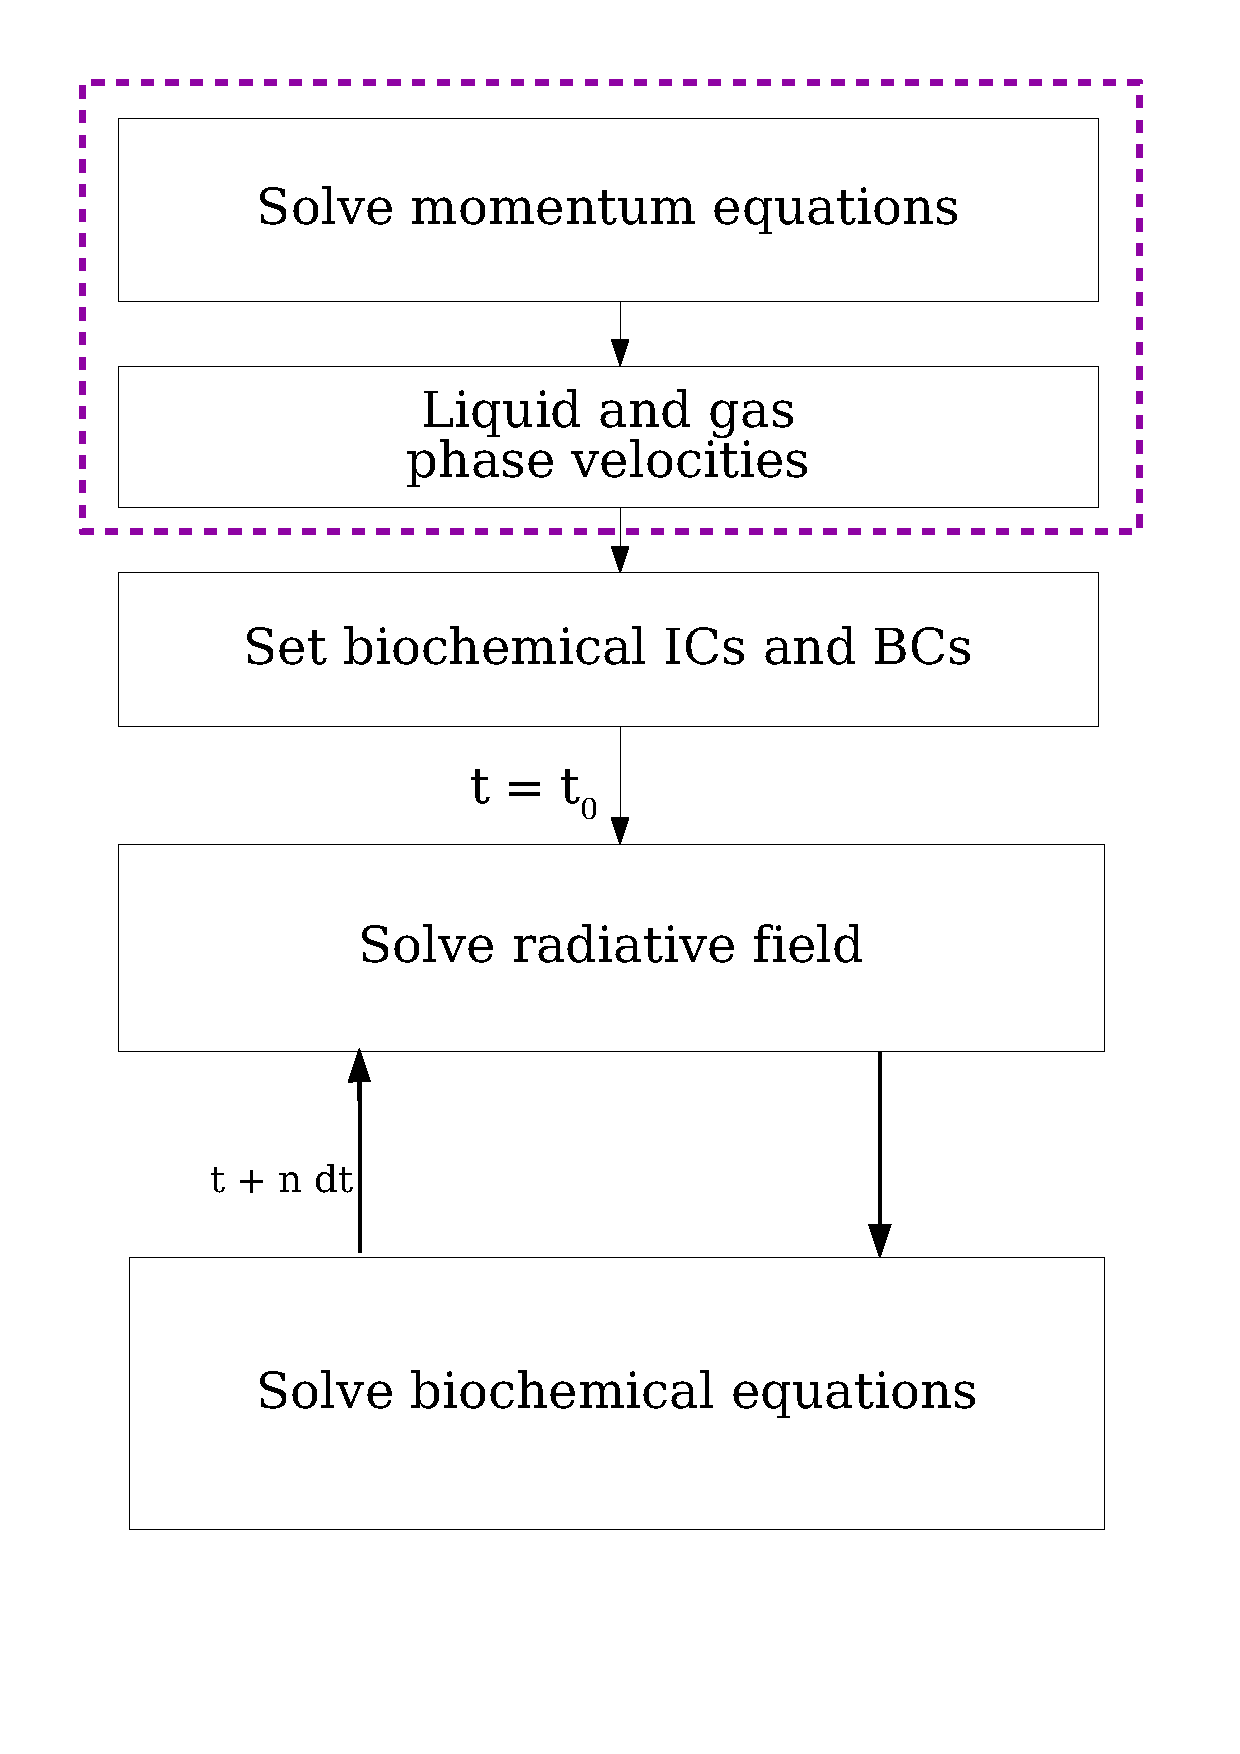
\includegraphics[width=0.6\linewidth]{Images/Chap3/algo_devt.pdf}
\caption{Solution algorithm for the solver. Momentum equations are solved until steady state is achieved and fed to the biochemical equation solver. The radiative field is updated every 15 minutes of simulated time.}
\label{fig:solnHierarchy}
\end{figure}

The flow field is solved first. The assumption that the solid species do not participate in the flow field can be made for PBRs which have relatively low total suspended solids concentrations compared with other activated sludge processes \cite{bitog2011}. The solver then enters a coupled radiation-biokinetics loop in which the radiative field is updated every 15 minutes of simulated time. A solution procedure that updated the radiative field at every time step was tested, but was prohibitively slow, and it was found to be unnecessary to update at such high frequency. Since the change in radiative properties due to biomass growth occur over an extended time frame, the update interval was found to not substantially influence the results.
\skippingparagraph

The solver used for these simulations is the \texttt{pamFoam} solver: a multiphase, multiphysics implementation of a finite volume hydrodynamics, radiation, and biokinetics solver, which is built upon version 5.0 of the OpenFOAM framework, a collection of C++ libraries for solving continuum mechanics problems \cite{theopenfoamfoundation2017}. The solver and run-time dictionaries have been released under the AGPL-3 license, and can be accessed online (https://gitlab.com/leboucher/pamFoam/tags/v5.1.0). The solver incorporates a custom radiation transport library built upon the finite volume discrete ordinates method \cite{raithby1990}, but adapted for use with phototrophic models. Its source code can also be found online (https://gitlab.com/leboucher/photoBio/tags/v5.1.0). The solid and soluble species were implemented as passive scalar transport equations.


%%%%%% RESULTS AND DISCUSSION

\section{Results and Discussion}
%The differences in characteristic time constants between enzymatic response ($10^{-6}\, s$), dynamic radiative field ($10\, s$) and microbial growth (hours or days) are multiple orders of magnitude. Therefore, when analysing PBR systems, the evolution of the radiative field due to microbial growth (order of hours), the dynamic radiative field (order of seconds), need to be considered. As the time scale of enzymatic response is low when compared to the other two phenomena, the associated effects do not require analysis. 

\subsection{Radiative field dynamics}

As the biomass grows in suspension over time, There is a decrease in intensity and distribution of the radiative field (Cf Eq. \ref{eq:rteSimplified}). This is shown in Fig.\ \ref{fig:rad_evol}(a). This demonstrates that despite a similar radiation intensity, the geometry of the FPR is better than the CR, resulting in a higher average irradiation intensity, and a greater attenuation over time due to faster biomass growth. Fig.\ \ref{fig:rad_evol} also shows spatial distribution of radiative intensity at the start of the simulation, and at 24 hours. Sub-figures b and c correspond to the FPR, and sub-figures d and e show the CR. This demonstrates a substantial attenuation over time from 12 $\mathrm{W m^{-2}}$ to 7 $\mathrm{W m^{-2}}$ in the FPR and from 5 $\mathrm{W m^{-2}}$ to 3 $\mathrm{W m^{-2}}$ in the CR. The percentage decrease corresponded to an increase in the phototrophic biomass $\mathrm{X_{PB}}$ from $\mathrm{0.5 \, g\, COD\, L^{-1}}$ to $\mathrm{1.0 \, g\, COD\, L^{-1}}$ in the FPR and $\mathrm{0.5 \, g\, COD\, L^{-1}}$ to $\mathrm{0.8 \, g\, COD\, L^{-1}}$ in the CR over the same period of 24 hours. The change in other particulate species was relatively small over that same time period. 

\begin{figure}[tp]
\centering
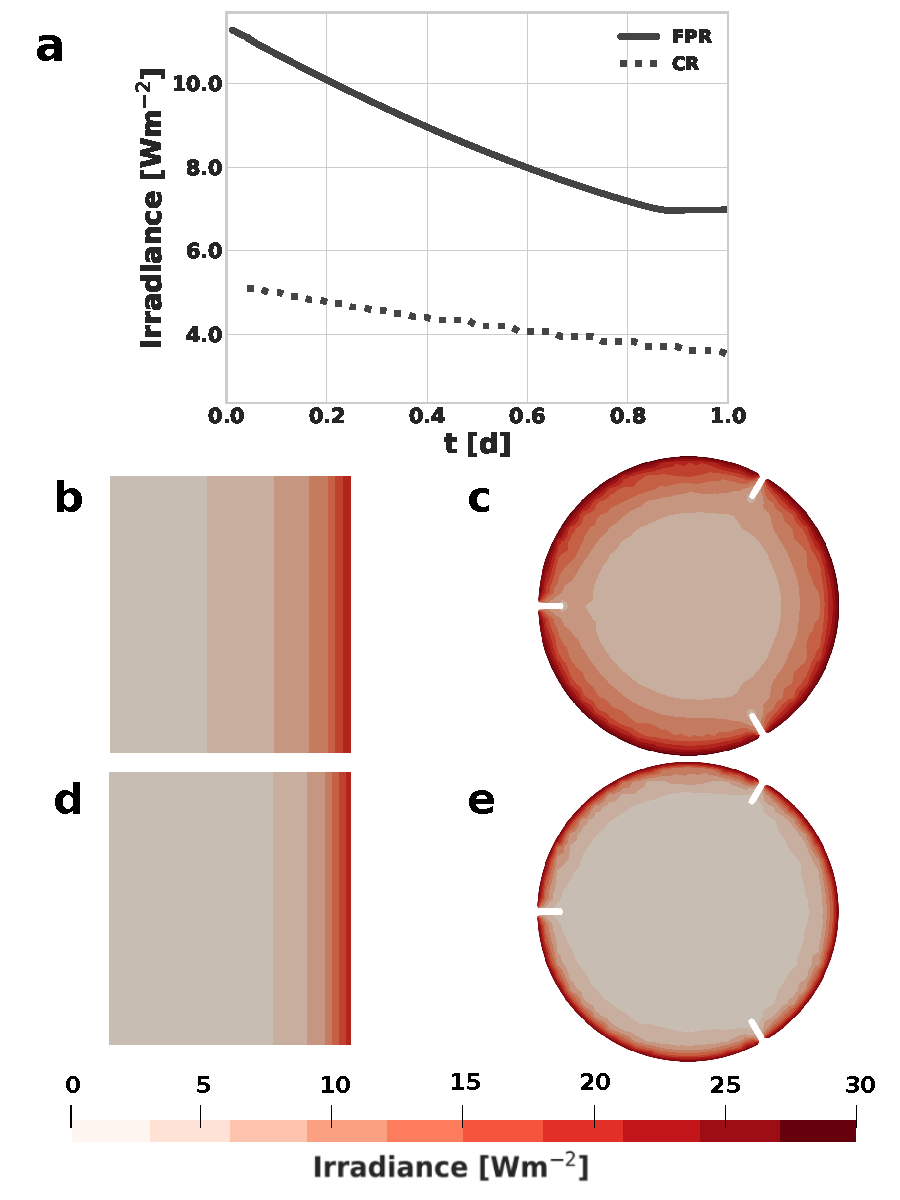
\includegraphics[scale=0.75]{Images/Chap3/rad_field_dynamics.pdf}
\caption{Evolution of the radiative field ($\mathrm{W m^{-2}}$), volume averaged over all time steps, and the spatial changes over time for the FPR and CR. Cross-sectional view at reactor from 0 cm to 3 cm from the radiation source. (b,c) corresponds to the radiative field at the start of the simulation, and (d,e) is the radiative field at 24 hours for the FPR and CR respectively.}
\label{fig:rad_evol}
\end{figure}

Findings from other studies \cite{kong2014} have shown that volumes within a reactor with an irradiance below $\mathrm{2\, Wm^{-2}}$ are effectively dark zones. Over time, self shading by biomass becomes apparent, which means that the fluid hydrodynamics become increasingly important if PBRs are to maintain substantial phototrophic biomass at high concentrations. For the FPR, the volume percentage of dark zones is 0\%, compared with 30\% for the CR. At 24 hours of simulated time, despite  25\% more particulate matter, only 25\% of the volume is in the dark, compared with 55\% for the CR. Both the limitations in nutrient and photon availability mean that this proportion sees diminishing rates of biomass shading as the simulation continues. These results support other findings that in suspended biomass PBRs, the majority of the reactor is in the dark when operating at steady state with substantial phototrophic biomass and particulate concentrations. It is clear that for near infrared radiation, attenuation is more significant within the phototrophic media than in the gas phase, and both multiphase (gas-liquid) and single phase liquid systems were modelled, although a more thorough investigation around the bubble dynamics and their effect on the radiative field is required to quantify these interactions.

\subsection{Short-term particle radiation dynamics}
\label{ssec:strf}
The short term particle radiation dynamics result from the fluid field moving biomass particles within the heterogeneous radiative field as shown in Fig. \ref{fig:G850_short}. The first column (a,c) corresponds to the particle radiation dynamics of the FPR, with the same data being represented as a dynamic plot (a) and a frequency histogram (c). The second shows the parallel results for the CR. This demonstrates that biomass in both reactors is subject to on-off irradiance cycles on the order of 3-5 s, with an amplitude of 20 $\mathrm{W m^{-2}}$. However, the dynamics are quite different, with particles in the FPR being irradiated for longer, and with a higher base-line (5 $\mathrm{W m^{-2}}$ in the FPR compared with 0 $\mathrm{W m^{-2}}$ in the CR). This indicates that in the FPR, particles are effectively always irradiated at a minimum level, whereas in the CR,  there is complete on-off cycling. 

\begin{figure}[tp]
\centering
%\hspace*{-2cm} 
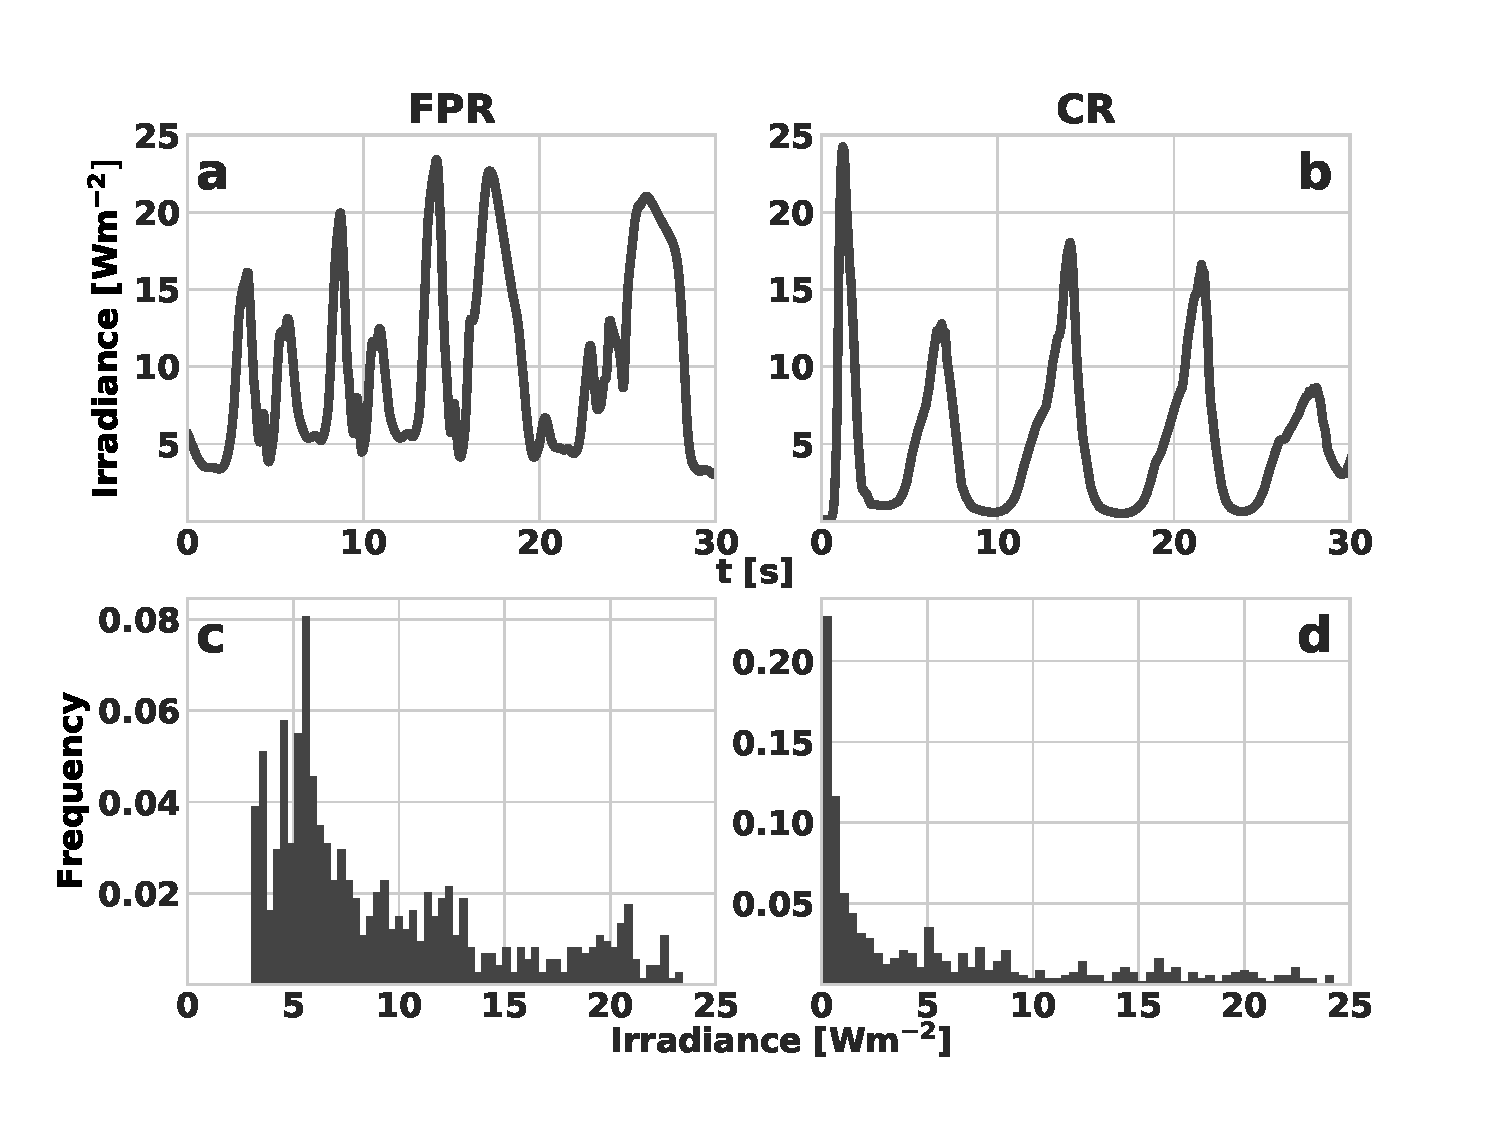
\includegraphics[width=1.\linewidth]{Images/Chap3/G850_short.pdf}
\caption{Particle radiation dynamics for an 850 nm band of irradiance. The top row (a, b) shows the transient radiative field experienced by a PPB particle for the FPR and CR reactors respectively. The same field is represented for both reactors (c, d) as a histogram on the bottom row. Both reactors have an incident irradiance of 30 $\mathrm{ W m^{-2}}$.}
\label{fig:G850_short}
\end{figure}

A question arising of the dynamic radiative field is whether the PPB biomass is sufficiently fast to respond to these changes. If the biomass response is much faster than the change in intensity, the growth kinetics can be treated as a continuous function (with dependence on intensity). If biomass response kinetics are also on the order of seconds, lower-level expressions would be required (which also consider photo-enzyme kinetics). The response time for \textit{Rhodobacter sphaeroides} was determined in the literature to be in the order of $10^{-11}$ seconds \cite{slouf2012}; a time constant much smaller than the periods seen in Fig. \ref{fig:G850_short}. Therefore, this justifies the use of a continuous function with respect to radiation for both this case, and in scaled-up systems, since they will generally have longer time constants due to the larger dimension with respect to velocity. This also justifies the approach used in this study to generate results, with biomass growth coupled to the radiative field, and phototrophic organisms self-shading as they grow.

\subsection{Growth of PPB biomass and uptake of soluble substrates}
\label{ssec:ppb_growth}
Four comparative simulations were done to assess the full Eulerian solution (as used so far in this study - solution 4) to three reduced continuously stirred tank reactor (CSTR) versions. These include (for each reactor):

\begin{enumerate}
    \item Uniform irradiance at incident value $\mathrm{30.0\, W\, m^{-2}}$ (ODE1). This is the standard approach that can be applied in a lumped-parameter model \cite{bechet2013}.
    \item Irradiance fixed at the the volume-averaged value as presented at in Fig. \ref{fig:rad_evol}(a). These values for the FPR and CR were $\mathrm{11\, W\, m^{-2}}$ and $\mathrm{5\, W\, m^{-2}}$ respectively (ODE2).
    \item Dynamic irradiance as determined and presented in Fig. \ref{fig:G850_short}(a, b). This data is treated as a dynamic input to the lumped parameter model (ODE3). The main reduction in extent compared to a full CFD simulation is that the biomass/substrate do not need to be represented by scalars. In order to represent the effect of only modelling the liquid-irradiance system, the 30 s profile was replicated in time to 24 h rather than taking the full dynamic profile which includes long-term temporal light attenuation due to biomass growth.
    \item Full Eulerian CFD solution (CFD).
\end{enumerate}

In the first two cases, no CFD is required, while in the latter two cases, CFD is required to identify the particle radiation exposure pattern, and for the integrated model respectively. The first two cases were explored because certain studies have taken modelling approaches using lumped parameters based on single values of uniform irradiance, with little information as to the spatial distribution of the radiative intensity field. This has been applied using either the surface incident exposure \cite{uyar2007, zhou2014}, or volume averaged irradiance \cite{molinagrima1996, bordel2009}. This can lead to an over-prediction when reporting growth rates.
\skippingparagraph
The biomass concentrations (in mgCOD/L) are shown for the various modelling approaches for both systems (Fig. \ref{fig:growth_evol}(a, b)). These demonstrate light-limited, fairly uniform growth rates towards the substrate depletion point where the growth stops (\textit{i.e.} a batch system). The uniform irradiance approaches generally over-predicted growth rates, particularly in the cylindrical reactor (where irradiation was fundamentally less efficient). The dynamic exposure approach was generally effective in representing biomass profiles, but with a clear deviation with respect to the full CFD approach. Specifically, there were slightly slower growth rates for ODE3 vs CFD. This is somewhat surprising since the final attenuation is higher in the full CFD approach when compared with ODE3 (due to biomass growth), but could be explained by the fact that this attenuation is due to biomass exposure rather than water attenuation. Therefore the light is not "lost", but rather used during attenuation.
\skippingparagraph
Fig. \ref{fig:growth_evol}(c-f) shows the uptake concentration of soluble substrates of the same simulations. Again, the hybrid approach (ODE3) is most effective compared with CFD, but there are substantial deviations for all three ODE approaches. The large deviations for substrate $\mathrm{S_{AC}}$ (Fig. \ref{fig:growth_evol}(c, e)) and $\mathrm{S_S}$ (Fig. \ref{fig:growth_evol}(d, f)) are most likely caused by inhibition of each respective uptake process (photoheterotrophic uptake for acetic acid, and for other organics) caused by the presence of the other soluble compound class. This, combined with the difference in uptake rates for acetate uptake ($\mathrm{2.4\, d^{-1}}$) and photoheterotrophic uptake ($\mathrm{1.4\, d^{-1}}$) \cite{puyol2017} mean that based on the amount of light available in the system, different behaviour can occur.  
\skippingparagraph
The full ODE approach (ODE1, ODE2), as stated above, is the most common approach, taking either surface irradiation \cite{uyar2007, zhou2014}, or an approximated reduced average irradiance \cite{lee1987, molinagrima1996, bordel2009}. This provided unsatisfactory results, particularly in the simplified CR. With respect to growth rates, and in an actual system, these variations would be absorbed by biochemical parameters, making them non-transferable to other systems. A system can only be effectively approximated with a lumped parameter modelling approach if the reactor is not only well mixed, but also well serviced with a uniform irradiance which can be measured effectively. This would likely not be an effective photobioreactor field design, but these factors also mean that some care must be taken even in laboratory systems when determining biological parameters, since the surface measured irradiance will almost certainly not be the \textit{in situ} irradiance. This would have an impact on biomass growth parameters. 

\begin{figure}[tp]
\centering
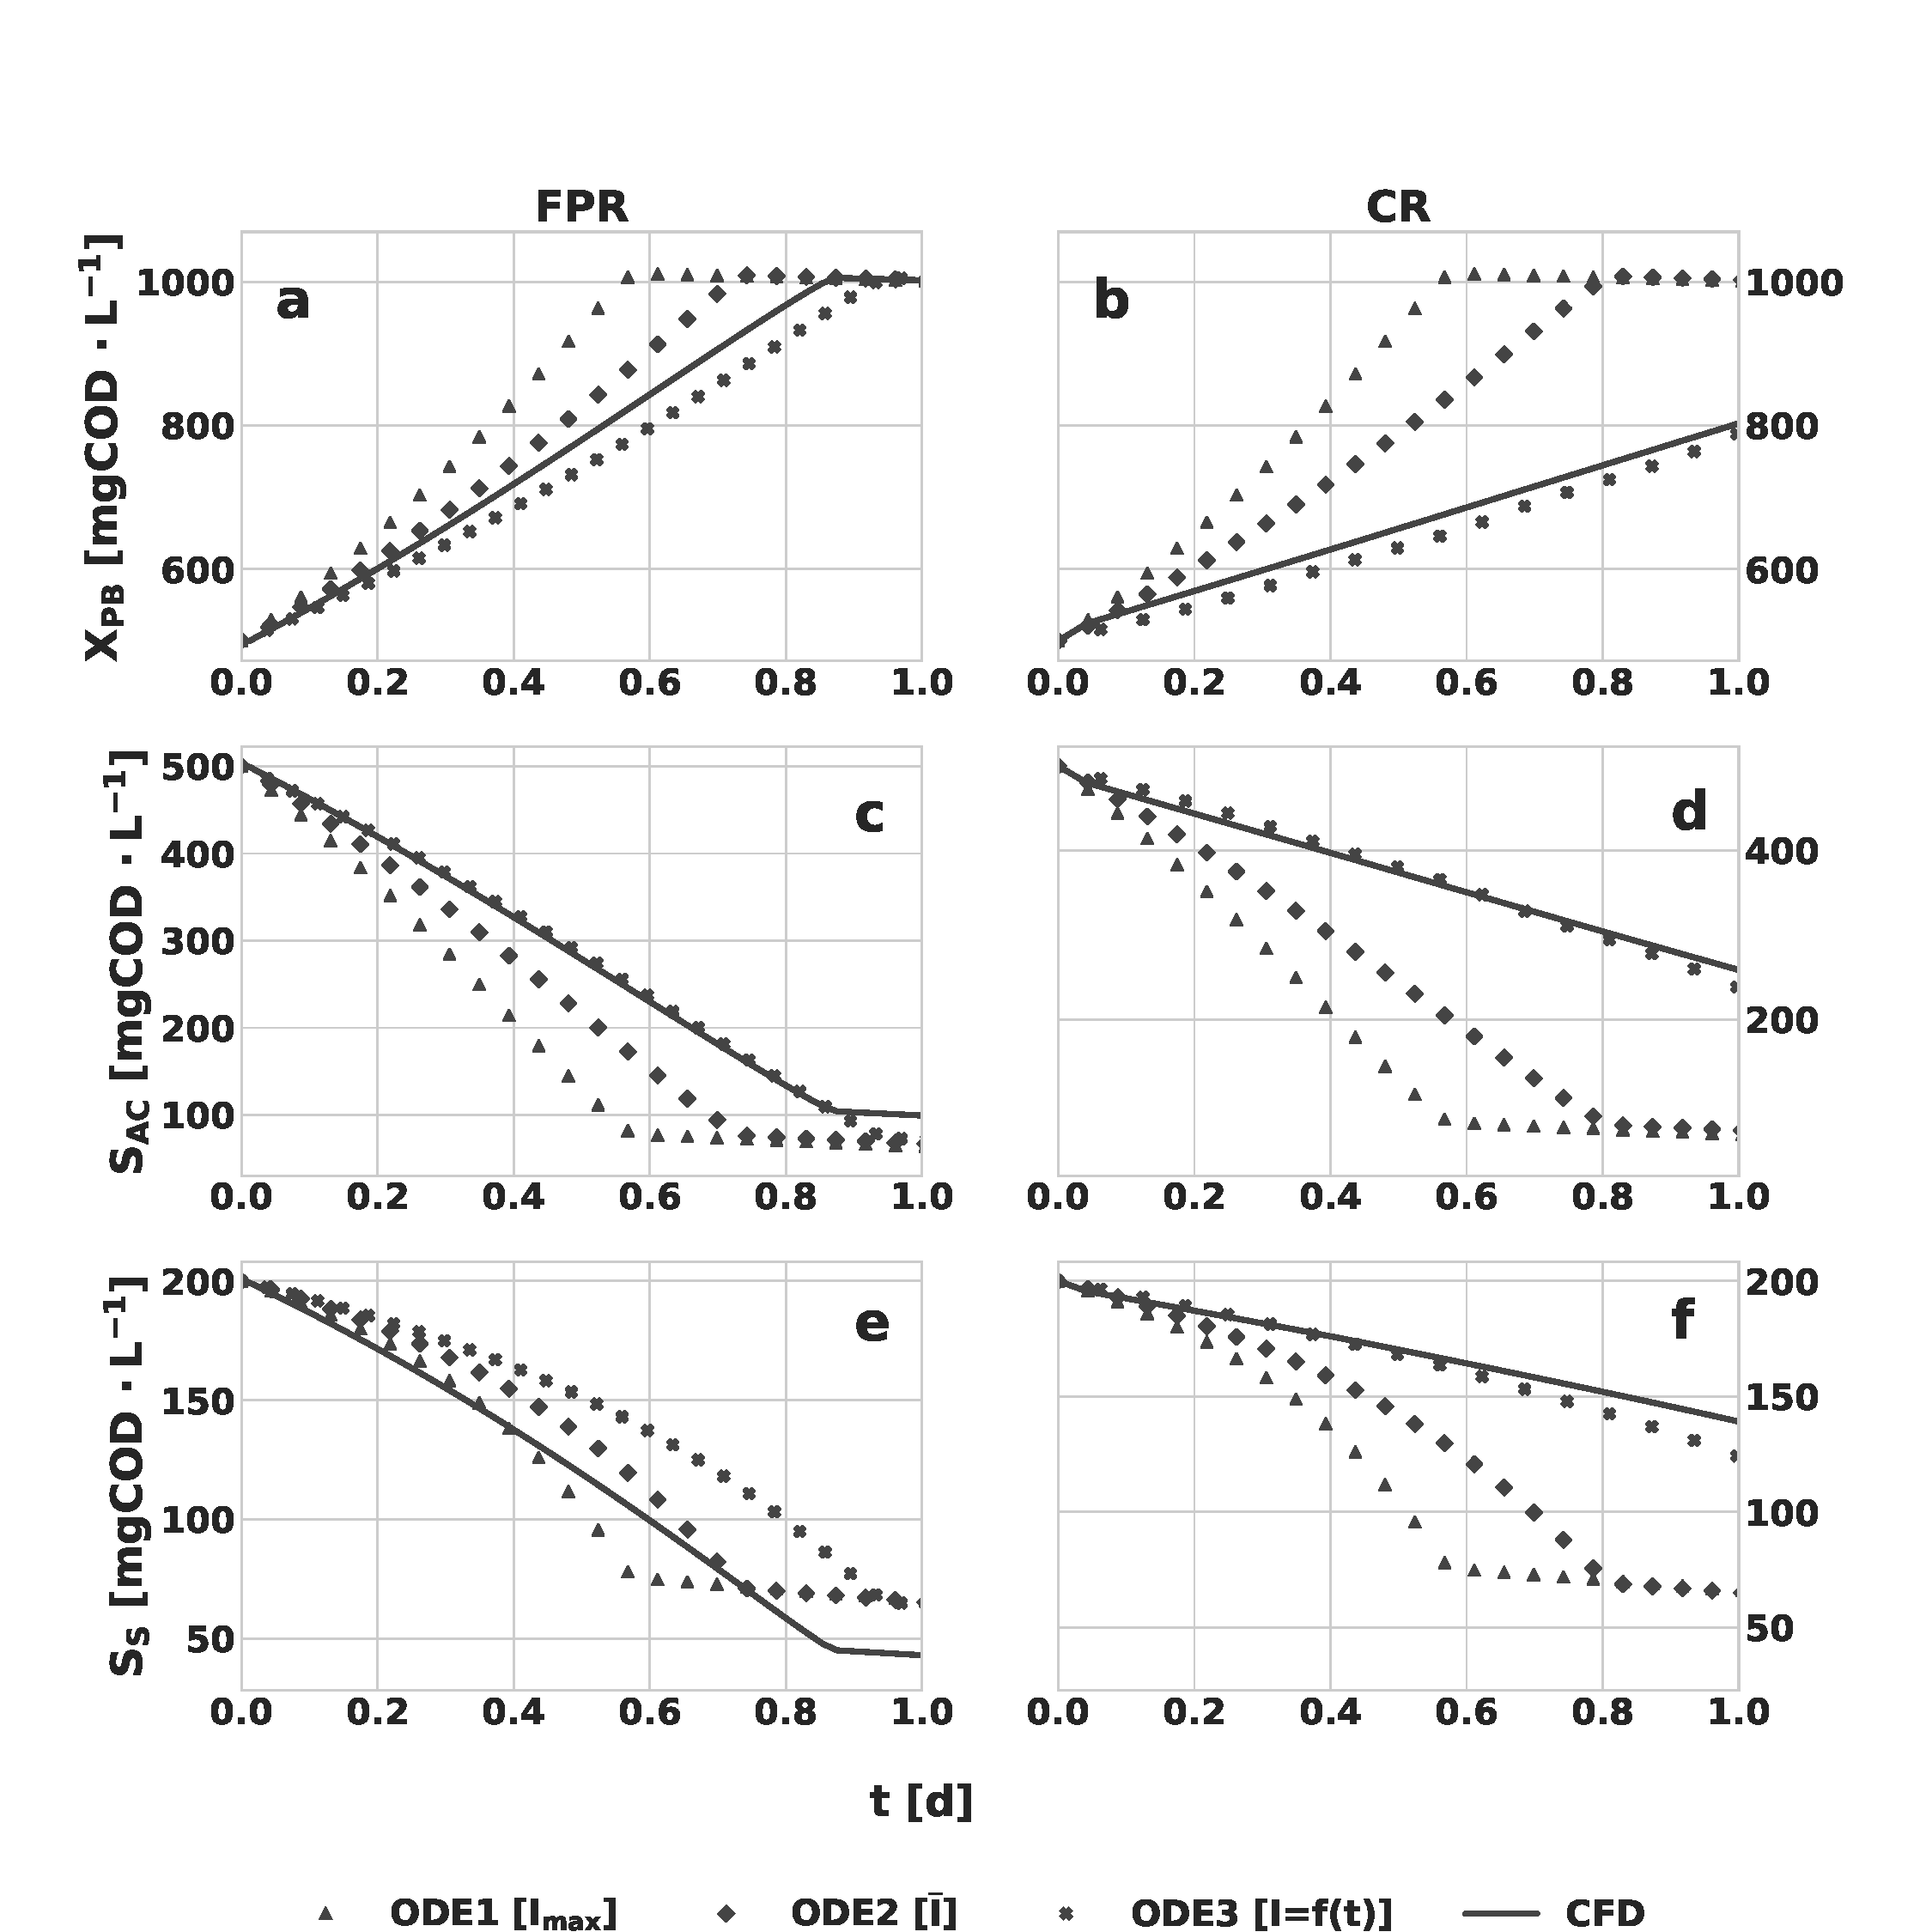
\includegraphics[scale=0.38]{Images/Chap3/growth_kinetics.pdf}
\caption{Biomass growth and substrate uptake for the FPR (a, c, e) and the CR (b, d, f). The first row shows the growth of PPB and the second and third rows show the consumption of acetic acid and other readily biodegradable soluble organics respectively. For all figures, the triangles correspond to ODE1, the diamonds correspond to ODE2, the the crosses represent ODE3, and the solid line is the CFD solution.}
\label{fig:growth_evol}
\end{figure}

The dynamic irradiance approach (ODE3) was far more effective in biological simulation, but the irradiance profile changes in each case, and cannot effectively represent irradiance changes as biomass experiences long-term growth. This has quite complex impacts, including potentially a loss in efficiency due to reduced biomass based attenuation. When compared with the full Eulerian solution (CFD), the dynamic irradiance solution has a slightly slower growth rate, but the time constant is similar for both simulations. The hybrid approach therefore has some value, particularly where a full model cannot be formulated. However, the full model provides complete interpretation at a modest increase in computational complexity. 

\subsection{Limitations of the model}
\label{ssec:limitations}
\subsubsection{CFD considerations}
There are three main limitations of the study with respect to the CFD implementation. Firstly, while gas and liquid phases have been modelled and biochemical state variables have been segregated in the liquid phase, the effect of biological activity on the gas field have not been incorporated. The mass transfer between phases was also not considered in this case. Including mass transfer models is important for photoautotrophic (gas fed) or photosynthetic ($\mathrm{CO_2}$) growth. Any mass transfer model is dependent on how the dispersed gas field is solved. Here, a uniform bubble Eulerian approach was taken, but an alternative that considers bubble size distribution such as population balance modelling could lead to an improvement in prediction of mass transfer. A better represented bubble size distribution would also allow analysis of its dynamic effects on the radiative field.  
This model considers planktonic biomass modelled as passive scalars. The momentum coupling would not substantially change interaction with the radiative field. However, an important possible extension is the inclusion of a spatially explicit biofilm. The current model lends itself well to include a continuum based biofilm model as a module in a broader continuum-based phototrophic growth model. 
\skippingparagraph
As the biomass has been implemented as passive scalars, the effects of changes in biomass concentration on the flow fields have not been quantified (\textit{i.e.}, does not affect rheology, density or momentum). This could be incorporated through an upgrade of the biomass from scalar to dispersed phase. Modelling the solid system in a Lagrangian framework can also link the particulate species with a set of physical information, such as particle density and diameter. The particulate species as they are currently modelled could also be linked to a particulate density, which would then have an effect on the flow field. 

\subsubsection{Biochemical system limitations}
This system differs from photosynthetic algae or cyanobacteria, where photosynthetic organisms may be in multiple states (excited, photoinhibited or resting) \cite{bechet2013}. The state depends on the radiative intensity and the light history of the organisms. In addition, nitrogen storage becomes an important factor \cite{bernard2011}. The short-term particle radiation dynamics as observed here are even more important in photosynthetic systems, where the transition in biological state adds another system dynamic which is on the same speed order as the cycling speed. Therefore, consideration of photo-dynamics is even more important when simulating white light systems, since, as discussed above, enzyme response is extremely fast (and photo-dynamics do not interact with this), while a change in photo-state is far slower. Photo-inhibition is another important factor not considered in the current model. The current system was irradiated with 30 $\mathrm{W m^{-2}}$, and photo-inhibition has been reported to start occurring closer to 900 $\mathrm{W m^{-2}}$ \cite{miyake1999}. Updating the model to include photo-inhibition terms would increase the range of applicability of the model to outdoor PBR systems, and is an important factor for white light systems as discussed above. The time constant for recovery from photo-inhibition may make this a more complex response function, and increase the importance of considering photo-dynamics. 
\skippingparagraph
This model was simulated looking at a single radiation band at 850 nm. In reality, the growth of PPB depends on other wavelength bands, including 375 nm and 590 nm (facultative carotenoids) and the near infrared band ranges from 830 nm to 900 nm \cite{overmann2006a}. Upgrading the biochemical model to include the growth on several different wavelengths would lead to resolution of important aspects, including increased and differential attenuation of higher energy radiation. However, assigning fixed behaviour to organisms which can adapt to different environmental conditions, such as the growth or loss of chromaphores due to low or high intensity radiative fields, means that there will always be a level of uncertainty which cannot be described by the model. 

%%%% Conclusions
\section{Conclusions}
This study has looked at two different reactor setups; a flat plate reactor (FPR) and a cylindrical reactor (CR). Over these two different reactor geometries, four modelling approaches were evaluated;
\begin{enumerate}
    \item ODE1: An ODE system taking a uniform radiative field equal to that of the incident irradiance.
    \item ODE2: An ODE system taking a uniform radiative field equal to its value halfway into the domain as solved by the radiative transfer equation here, or alternatively by a Beer-Lambert relationship.
    \item ODE3: An ODE system taking as input a dynamic irradiance experienced by a particle as it is carried by the velocity field in the reactors.
    \item CFD: A full Eulerian CFD approach accounting for fluid flows, radiative transfer, and the system of biochemical equations for purple phototrophic bacteria.
\end{enumerate}

The first two approaches tended to over-predict growth rates, meaning that the spatial variations within PBRs are important to consider, and local effects can have an impact on the overall solution. The results for ODE3 were similar to those for the full Eulerian CFD solution, irrespective of reactor geometry. This approach presents an appropriate compromise when computational resources are scarce, however the full Eulerian approach provides the complete interpretation for the PBR systems, with scope to expand on this model with more physical processes. 
\skippingparagraph
Several limitations to the study were identified, and were classed in two categories; CFD limitations and biochemical modelling limitations. The CFD limitations were that mass transfer in multiphase systems was not solved, and the model was developed as a planktonic model with passive scalars, limiting the description of physical processes such as biofilm development and effects on the flow field due to changes in density. The biochemical limitations extended on previous work to highlight the adaptive changes of pigment production in response to the radiative field, and the effects of photoinhibition on uptake rates.
%CFD including photo-attenuation identified that particles were subject to both short and long-term irradiative dynamics, the former due to cycling through light-dark regions, and the latter due to overall biomass growth. A biologically coupled CFD solution versus uniform irradiance ODE approaches (as commonly applied) found the latter could not effectively predict dynamics of growth in batch. A compromise (which identified particle irradiation dynamics from non-coupled CFD) was effective, but the computational effort approached the full CFD method.

%\section*{Acknowledgements}
%The authors would like to thank Domenico Santoro and the team at Trojan Technologies, London, Canada, for their help with CFD simulations for photobiological systems. This work was funded by the CRC for Water Sensitive Cities (project C2.1). Christopher De Groot acknowledges funding from the Natural Sciences and Engineering Research Council of Canada (NSERC) [RGPIN-2017-04078].

%\section*{Appendix. Supplementary material}
%Supplementary material has been provided with this work \\(DOI: 10.6084/m9.figshare.7459106.v2). In addition, the model codes can be found at https://gitlab.com/leboucher/pamFoam/tags/v5.1.0 for the solver, and https://gitlab.com/leboucher/photoBio/tags/v5.1.0 for the \texttt{photoBio} library. 
